%%%%%%%%%%%%%%%%%%%%%%%%%%%%%%%%%%%%%%%%%%%%%%%%%%%%%%%%%%%%%%%%%%%%%%%%%%%%%%%%%%%%%%%%
% Talk/Seminar/Event flyer
%
% LaTeX Template
% Version 1.0 (02/02/2023)
%
% Author: Alberto Cuadra Lara (acuadra@ing.uc3m.es) - acuadralara.com
%
% License: CC BY-NC-SA 4.0 (http://creativecommons.org/licenses/by-nc-sa/4.0/)
%
% Important note: this template needs to be compiled with XeLaTeX
%%%%%%%%%%%%%%%%%%%%%%%%%%%%%%%%%%%%%%%%%%%%%%%%%%%%%%%%%%%%%%%%%%%%%%%%%%%%%%%%%%%%%%%%

%%%%%%%%%%%%%%%%%%%%%%%%%%%%%%%%%%%%%%%%%%%%%%%%%%%%%%%%%%%%%%%%%%%%%%%%%%%%%%%%%%%%%%%%
% Document setup and packages
%%%%%%%%%%%%%%%%%%%%%%%%%%%%%%%%%%%%%%%%%%%%%%%%%%%%%%%%%%%%%%%%%%%%%%%%%%%%%%%%%%%%%%%%
% Set document class: paper size, font size and orientation
\documentclass[a4paper,12pt,landscape]{article} 
% Set margins
\usepackage[left=11mm, right=11mm, top=11mm, bottom=11mm]{geometry}
% Load packages to change fonts and use icons
\usepackage{fontspec, fontawesome5, academicons}
% Set main font (default: rasa) and font path (default: fonts/)
\defaultfontfeatures{Mapping=tex-text}
\setmainfont[
    Path = fonts/,
    BoldFont={Rasa-Bold.ttf}, 
    ItalicFont={Rasa-BoldItalic.ttf},
    BoldItalicFont={Rasa-Italic.ttf}
 ]{Rasa-VariableFont_wght.ttf}
% Load Formatting package
\usepackage{parskip}
% Load Tikz packages
\usepackage{tikz}
\usepackage{tikzpagenodes}
\usetikzlibrary{calc}
% Load package to use links
\usepackage[hidelinks, breaklinks]{hyperref}
% Load colors package
\usepackage{tcolorbox}
% Define colors
\definecolor{red}{rgb}{0.5765,0.0902,0.1765}
\definecolor{blue}{RGB}{87,145,179}
\definecolor{mycolorbox}{RGB}{15, 61, 77}
% Set color box
\newtcolorbox{mybox2}{colback=mycolorbox!5!white, colframe=mycolorbox!75!black}
% Set background color
\pagecolor{mycolorbox!3!white}

%%%%%%%%%%%%%%%%%%%%%%%%%%%%%%%%%%%%%%%%%%%%%%%%%%%%%%%%%%%%%%%%%%%%%%%%%%%%%%%%%%%%%%%%
% Document
%%%%%%%%%%%%%%%%%%%%%%%%%%%%%%%%%%%%%%%%%%%%%%%%%%%%%%%%%%%%%%%%%%%%%%%%%%%%%%%%%%%%%%%%
\begin{document}
% Removes page numbering
\pagestyle{empty}
%%%%%%%%%%%%%%%%%%%%%%%%%%%%%%%%%%%%%%%%%%%%%%%%%%%%%%%%%%%%%%%%%%%%%%%%%%%%%%%%%%%%%%%%
% Column 1 - abstract
%%%%%%%%%%%%%%%%%%%%%%%%%%%%%%%%%%%%%%%%%%%%%%%%%%%%%%%%%%%%%%%%%%%%%%%%%%%%%%%%%%%%%%%%
\begin{minipage}[c]{0.5\textwidth}
    \vspace{0.55cm}
    % Title
    \section*{Development of an open-source thermochemical code: Fundamentals and application to shock turbulence interaction problems in the hypersonic regime}
    % Decription
    In this seminar, we present the development of an in-house thermochemical code ---hereafter referred to as Combustion Toolbox (CT)--- for the solution of problems that involve chemical equilibrium of gas- and condensed-phase species. The thermochemical properties are computed under the ideal gas approximation using an up-to-date version of NASA’s 9-coefficient polynomial fits. CT is programmed in MATLAB with a modular architecture composed of three main modules: CT-EQUIL, CT-SD and CT-ROCKET. The core module, CT-EQUIL, minimizes the Gibbs/Helmholtz free energy of the system, upon the condition that the mixture properties are defined by two functions of state. CT-SD solves processes that involve strong changes in the dynamic pressure, such as steady shock and detonation waves under both normal and oblique incidence angles within the limits of regular shock reflections. Finally, CT-ROCKET estimates rocket engine performance under ideal conditions. The new tool is equipped with a versatile Graphical User Interface.\vspace{0.23cm}

    We will also introduce a theoretical work based on the thermochemical effects of hypersonic shock waves interacting with weak turbulence in air. The problem begins with the prediction, based on first principles only, of the Hugoniot curve when the shock triggers vibrational excitation and molecular dissociation in a single-species diatomic gas. CT is used to extend this theory to include further effects, such as dissociation, ionization and recombination in multi-species ideal gas mixtures. The post-shock gas properties are then used to compute the turbulent amplification across the shock using linear interaction analysis (LIA). The LIA results presented here for air indicate that the enstrophy, anisotropy, intensity, and turbulent kinetic energy (TKE) of the fluctuations are more amplified through the shock than in the thermochemical frozen case. Moreover, the turbulent Reynolds number is also amplified across the shock at hypersonic Mach numbers in the presence of dissociation and vibrational excitation, as opposed to the attenuation observed in the thermochemical frozen case. Multi-species effects reshape the TKE curve by rendering two maxima that fit fairly well within the O$_2$ and N$_2$ dissociation processes.
    
\end{minipage}
\hfill
%%%%%%%%%%%%%%%%%%%%%%%%%%%%%%%%%%%%%%%%%%%%%%%%%%%%%%%%%%%%%%%%%%%%%%%%%%%%%%%%%%%%%%%%
% Column 2 - Time of the event and bio of the presenter
%%%%%%%%%%%%%%%%%%%%%%%%%%%%%%%%%%%%%%%%%%%%%%%%%%%%%%%%%%%%%%%%%%%%%%%%%%%%%%%%%%%%%%%%
\begin{minipage}[c]{0.44\textwidth}
    % Set logo of the host center
    \hfill
\includegraphics[width=0.55\linewidth]{figures/logo_unisalento.png}
    \newline
    % Set time of the event
    \begin{center}
        \begin{large}
            \begin{tabular}{r l}
                Time:     & \textbf{Feb, 15th (Wednesday), 2023}\\
                          & \textbf{8:30 am (San Francisco, GMT-8)}\\
                          & \textbf{5:30 pm (Rome, GMT+1)}\\
                Location: & \href{https://teams.microsoft.com/l/meetup-join/19%3ameeting_NWI4MGZjMzktOGIxZS00M2IzLTk1ZjgtZDgwMDViZjY0ZDVm%40thread.v2/0?context=%7b%22Tid%22%3a%228d49eb30-429e-4944-8349-dee009bdd7da%22%2c%22Oid%22%3a%225ab8b11d-d3b3-4361-8192-01d3a2a326e2%22%7d}{\underline{\textbf{\color{blue}Click here to join the seminar}}}
            \end{tabular}
        \end{large}
    \end{center}
    \vspace{0.5cm}
    \begin{mybox2}
    % Include picture of the presenter
    \begin{tikzpicture}
        \clip ($(current page text area.north east)!0.07!(current page text area.south east)!0.125!(current page text area.north west)$)
        circle (2.1cm) node {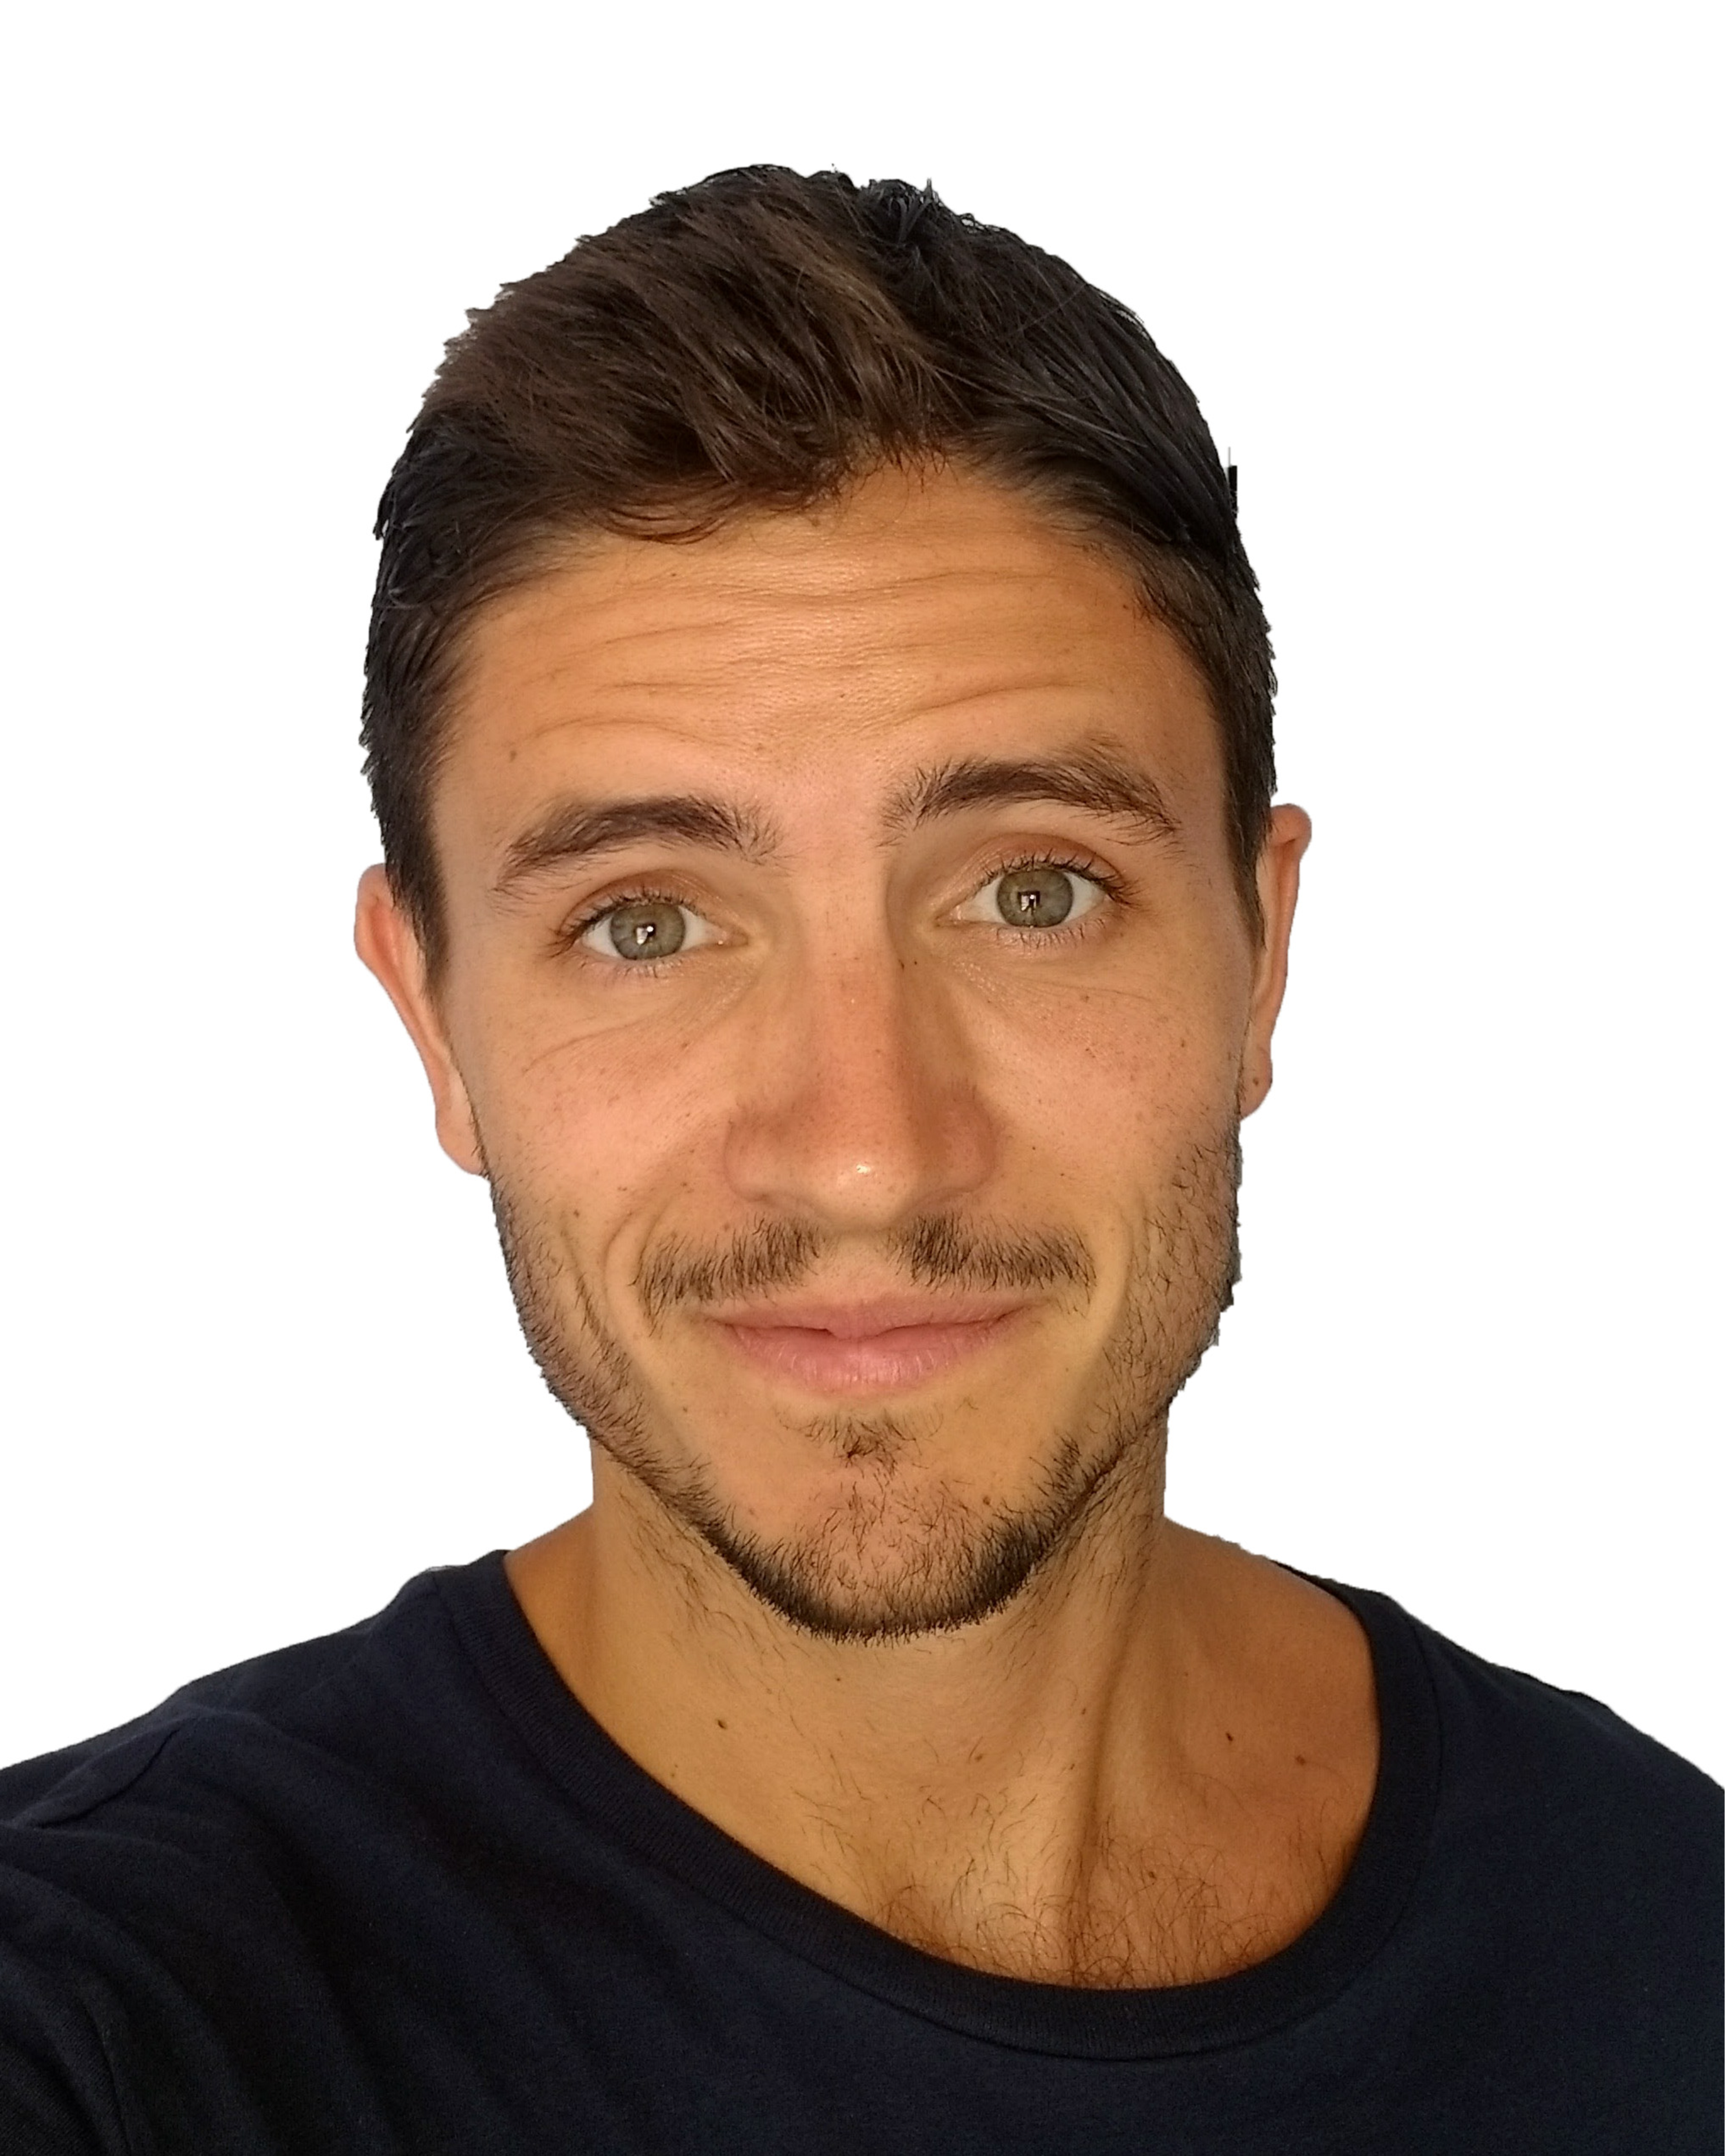
\includegraphics[width=0.35\linewidth]{figures/avatar.pdf}};
    \end{tikzpicture}
    % Include logo of the company of the presenter, name and position
    \begin{tikzpicture}[overlay]
        \node at (3.6, 3.2) {
\includegraphics[width=0.5\linewidth]{figures/logo_uc3m.pdf}};
        \node at (3.6, 1.5) {\Large \textbf{Alberto Cuadra}};
        \node at (3.6, 0.85) {\large Ph.D. fellow};
    \end{tikzpicture}
    % Include contact information of the presenter
    \begin{center}
        \begin{tabular}{rll}
            \textcolor{mycolorbox}{\faIcon{phone-alt}} & (+34) 91 624 8367 & \href{https://github.com/AlbertoCuadra}{\textcolor{mycolorbox}{{\faIcon{github}}} \  AlbertoCuadra}\\ 
            \textcolor{mycolorbox}{\faIcon{envelope}} & \href{mailto:acuadra@ing.uc3m.es}{acuadra@ing.uc3m.es} & \href{https://www.researchgate.net/profile/Alberto-Cuadra-Lara}{\textcolor{mycolorbox}{{\faIcon{researchgate}}} \  Alberto-Cuadra-Lara}\\
            \textcolor{mycolorbox}{\faIcon{external-link-alt}} & \href{https://acuadralara.com/}{acuadralara.com} &   \href{https://orcid.org/0000-0001-8280-2426}{\textcolor{mycolorbox}{{\aiOrcid}} \  0000-0001-8280-2426}
        \end{tabular}
    \end{center}
    \vspace{0.5cm}
    % Include bio of the presenter
    Alberto Cuadra received his 4-year degree in Industrial Engineering at Universidad de Málaga in 2017. He earned his MSc in Applied Mathematics at Universidad Carlos III de Madrid (UC3M) in 2019. Currently a Ph.D. fellow at UC3M under the supervision of Prof. Marcos Vera and Prof. César Huete at UC3M. His current research mainly focuses on two parts: the development of an open-source wider-scope thermochemical code, and the theoretical study of shock and detonations that travel along non-uniform conditions.
    \end{mybox2}
\end{minipage}
\end{document}